\documentclass[12pt,aspectratio=1610]{beamer}
\RequirePackage{
    amsmath,
    amssymb,
    calc,
    cancel,
    booktabs,
    color,
    siunitx,
    tikz,
    wrapfig,
    array,
    leftidx,
    float,
    etoolbox,
    fancyhdr,
    longtable,
    hyperref,
    ltcaption,
    ulem,
    wasysym,
    accents,
    listings,
    tabularx,
}

\hypersetup{
    hidelinks,
    breaklinks              = true,
}

\usepackage[final]{pdfpages}
\usepackage[many]{tcolorbox}

\RenewDocumentCommand{\vec}{m}{\mathbf{#1}}

\makeatletter
    \def\new@mathgroup{\alloc@8\mathgroup\mathchardef\@cclvi}
    \patchcmd{\document@select@group}{\sixt@@n}{\@cclvi}{}{}
    \patchcmd{\select@group}{\sixt@@n}{\@cclvi}{}{}
\makeatother

\RequirePackage{mathspec}                                   % includes fontspec
\RequirePackage{polyglossia}                                % multi-language support
\RequirePackage{xunicode}
\setdefaultlanguage{slovak}

% Setup fonts -- see fontspec/mathspec documentation.
\defaultfontfeatures{
    Mapping         = tex-text,
    Scale           = MatchLowercase,
    Ligatures       = TeX
}


\NewDocumentCommand{\labelmath}{m +m}{%
    \begin{equation}%
        #2%
        \label{#1}%
    \end{equation}%
}

\NewDocumentCommand{\labelalign}{m +m}{%
    \begin{align}%
        #2%
        \label{#1}%
    \end{align}%
}

\linespread{1.0}
\setlength{\parindent}{0cm}
\setlength{\parskip}{6pt}
\setlength{\abovedisplayskip}{0mm}
\setlength{\belowdisplayskip}{0mm}
\setlength{\abovedisplayshortskip}{0mm}
\setlength{\belowdisplayshortskip}{0mm}
\setlength{\itemindent}{0pt}
\setlength{\textfloatsep}{0mm}
\setlength{\tabcolsep}{3mm}
\setlength{\LTcapwidth}{0.8\textwidth}
\renewcommand{\arraystretch}{1.2}

\setcounter{secnumdepth}{2}

/home/kvik/dgs/core/tex/math.tex
\DeclareSIUnit\au{AU}
\DeclareSIUnit\pixel{px}
\DeclareSIUnit\lightyear{ly}
\DeclareSIUnit\parsec{pc}
\DeclareSIUnit\earthmass{M_{\earth}}
\DeclareSIUnit\speedoflight{c}
\DeclareSIUnit\foe{foe}
\DeclareSIUnit\year{yr}
\DeclareSIUnit\eur{€}
\DeclareSIUnit\solarmass{M_{\astrosun}}
\DeclareSIUnit\solarluminosity{L_{\astrosun}}
\DeclareSIUnit{\byte}{B}




\linespread{1.0}
\setlength{\parindent}{0cm}
\setlength{\parskip}{6pt}
\setlength{\abovedisplayskip}{0mm}
\setlength{\belowdisplayskip}{0mm}
\setlength{\abovedisplayshortskip}{0mm}
\setlength{\belowdisplayshortskip}{0mm}
\setlength{\itemindent}{0pt}
\setlength{\textfloatsep}{0mm}
\setlength{\tabcolsep}{3mm}
\renewcommand{\arraystretch}{1.2}

\setcounter{secnumdepth}{0}

\NewDocumentCommand{\fspicture}{m O{W} O{black}}{
    {
        \setbeamertemplate{navigation symbols}{}
        \setbeamercolor{background canvas}{bg = #3}
        \begin{frame}[plain]
            \begin{tikzpicture}[remember picture, overlay]
                \node[at=(current page.center)] {
                    \ifstrequal{H}{#2}{                                  
                        \includegraphics[height=\paperheight]{#1}%
                    }{%
                        \includegraphics[width=\paperwidth]{#1}%
                    }
                };
            \end{tikzpicture}
        \end{frame}
    }
}

\NewDocumentCommand{\frejm}{m +m}{
    \begin{frame}
        \frametitle{#1}
        #2
    \end{frame}
}

\NewDocumentCommand{\fragfrejm}{m +m}{
    \begin{frame}[fragile]
        \frametitle{#1}
        #2
    \end{frame}
}

\defbeamertemplate{description item}{align center}{\hfill\insertdescriptionitem\hfill}
\definecolor{desc}{rgb}{0.66, 0, 0}
\definecolor{citem}{rgb}{0.72, 0, 0}
\definecolor{csitem}{rgb}{0.90, 0, 0}
\definecolor{cssitem}{rgb}{1, 0.1, 0.1}
\definecolor{qprimarybg}{rgb}{0.95, 0.95, 0.95}
\definecolor{check}{rgb}{0, 0.8, 0}
\definecolor{coded}{rgb}{0.9, 0.9, 0.9}
\definecolor{todo}{rgb}{1.0, 0.3, 0.3}
\definecolor{model}{rgb}{0.75, 0, 0}

\setbeamertemplate{navigation symbols}{}
\newfontfamily{\semibold}{Segoe UI Semibold}
\RenewDocumentCommand{\emph}{m}{{\semibold#1}}
\NewDocumentCommand{\code}{m}{\textcolor{desc}{\texttt{#1}}}
\NewDocumentCommand{\model}{m}{\colorbox{coded}{\textcolor{model}{\texttt{#1}}}}
\NewDocumentCommand{\todo}{m}{\colorbox{todo}{#1}}

\mode<presentation> {
    \usetheme{Szeged}
    \usecolortheme{beaver}
    
    \usefonttheme{professionalfonts}
    \setallmainfonts{Minion Pro}
    \setmathrm{Minion Pro}
    
    \setsansfont{Segoe UI}
    \setmonofont{Consolas}
    \setbeamercolor*{enumerate item}{fg = citem}
    \setbeamercolor*{enumerate subitem}{fg = csitem}
    \setbeamercolor*{enumerate subsubitem}{fg = cssitem}
    \setbeamercolor*{description item}{fg = desc}
    \setbeamercolor*{itemize item}{fg = citem}
    \setbeamercolor*{itemize subitem}{fg = csitem}
    \setbeamercolor*{itemize subsubitem}{fg = cssitem}
    \setbeamercolor*{palette primary}{fg = red, bg = qprimarybg}
}

\newcommand<>\highlightbox[2]{%
    \alt#3{\makebox[\dimexpr\width-2\fboxsep]{\colorbox{#1}{#2}}}{#2}%
}

\AtBeginSection[]{
    \subsection{\insertsection}
    \begin{frame}
        \vfill
        \centering
        \begin{beamercolorbox}[sep = 18pt, center, shadow = true, rounded = true]{title}
            \usebeamerfont{title}\insertsectionhead%
            \vfill
        \end{beamercolorbox}
        \vfill
    \end{frame}
}

\makeatletter
% Render percent sign with nice font, not ugly Computer modern
    \mathcode`\%="7025

% Fixes mathspec bug -- URL numbers are rendered with wrong font
    \ernewcommand\eu@MathPunctuation@symfont{Latin:m:n}
    \DeclareMathSymbol{,}{\mathpunct}{\eu@MathPunctuation@symfont}{`,}
    \DeclareMathSymbol{?}{\mathpunct}{\eu@MathPunctuation@symfont}{`?}
    \DeclareMathSymbol{.}{\mathord}{\eu@MathPunctuation@symfont}{`.}
    \DeclareMathSymbol{<}{\mathrel}{\eu@MathPunctuation@symfont}{`<}
    \DeclareMathSymbol{>}{\mathrel}{\eu@MathPunctuation@symfont}{`>}
    \DeclareMathSymbol{/}{\mathord}{\eu@MathPunctuation@symfont}{`/}
    \DeclareMathSymbol{;}{\mathpunct}{\eu@MathPunctuation@symfont}{`;}
    \DeclareMathSymbol{(}{\mathopen}{\eu@DigitsArabic@symfont}{`(}
    \DeclareMathSymbol{)}{\mathclose}{\eu@DigitsArabic@symfont}{`)}
    \XeTeXDeclareMathSymbol{^^^^2026}{\mathinner}{\eu@MathPunctuation@symfont}{"2026}[\mathellipsis]
    \DeclareMathSymbol{0}{\mathalpha}{\eu@DigitsArabic@symfont}{`0}
    \DeclareMathSymbol{1}{\mathalpha}{\eu@DigitsArabic@symfont}{`1}
    \DeclareMathSymbol{2}{\mathalpha}{\eu@DigitsArabic@symfont}{`2}
    \DeclareMathSymbol{3}{\mathalpha}{\eu@DigitsArabic@symfont}{`3}
    \DeclareMathSymbol{4}{\mathalpha}{\eu@DigitsArabic@symfont}{`4}
    \DeclareMathSymbol{5}{\mathalpha}{\eu@DigitsArabic@symfont}{`5}
    \DeclareMathSymbol{6}{\mathalpha}{\eu@DigitsArabic@symfont}{`6}
    \DeclareMathSymbol{7}{\mathalpha}{\eu@DigitsArabic@symfont}{`7}
    \DeclareMathSymbol{8}{\mathalpha}{\eu@DigitsArabic@symfont}{`8}
    \DeclareMathSymbol{9}{\mathalpha}{\eu@DigitsArabic@symfont}{`9}
\makeatother


\title{Investigation of meteor models with numerical simulation}
\subtitle{Toying with models of meteor flight for a deeper understanding}
\author{\small \emph{Martin Baláž}\textsuperscript{1} \and Juraj Tóth, PhD.\textsuperscript{1} \and Peter Vereš, PhD.\textsuperscript{2} \\[4mm] \scriptsize
    \textsuperscript{1}Comenius University \\
    \textsuperscript{2}Minor Planet Center, Harvard-Smithsonian Center for Astrophysics}
\institute{IMC 2019, Bollmannsruh \& DAA colloquium}
\date{2019--10--09}

\begin{document}
    {
        \usebackgroundtemplate{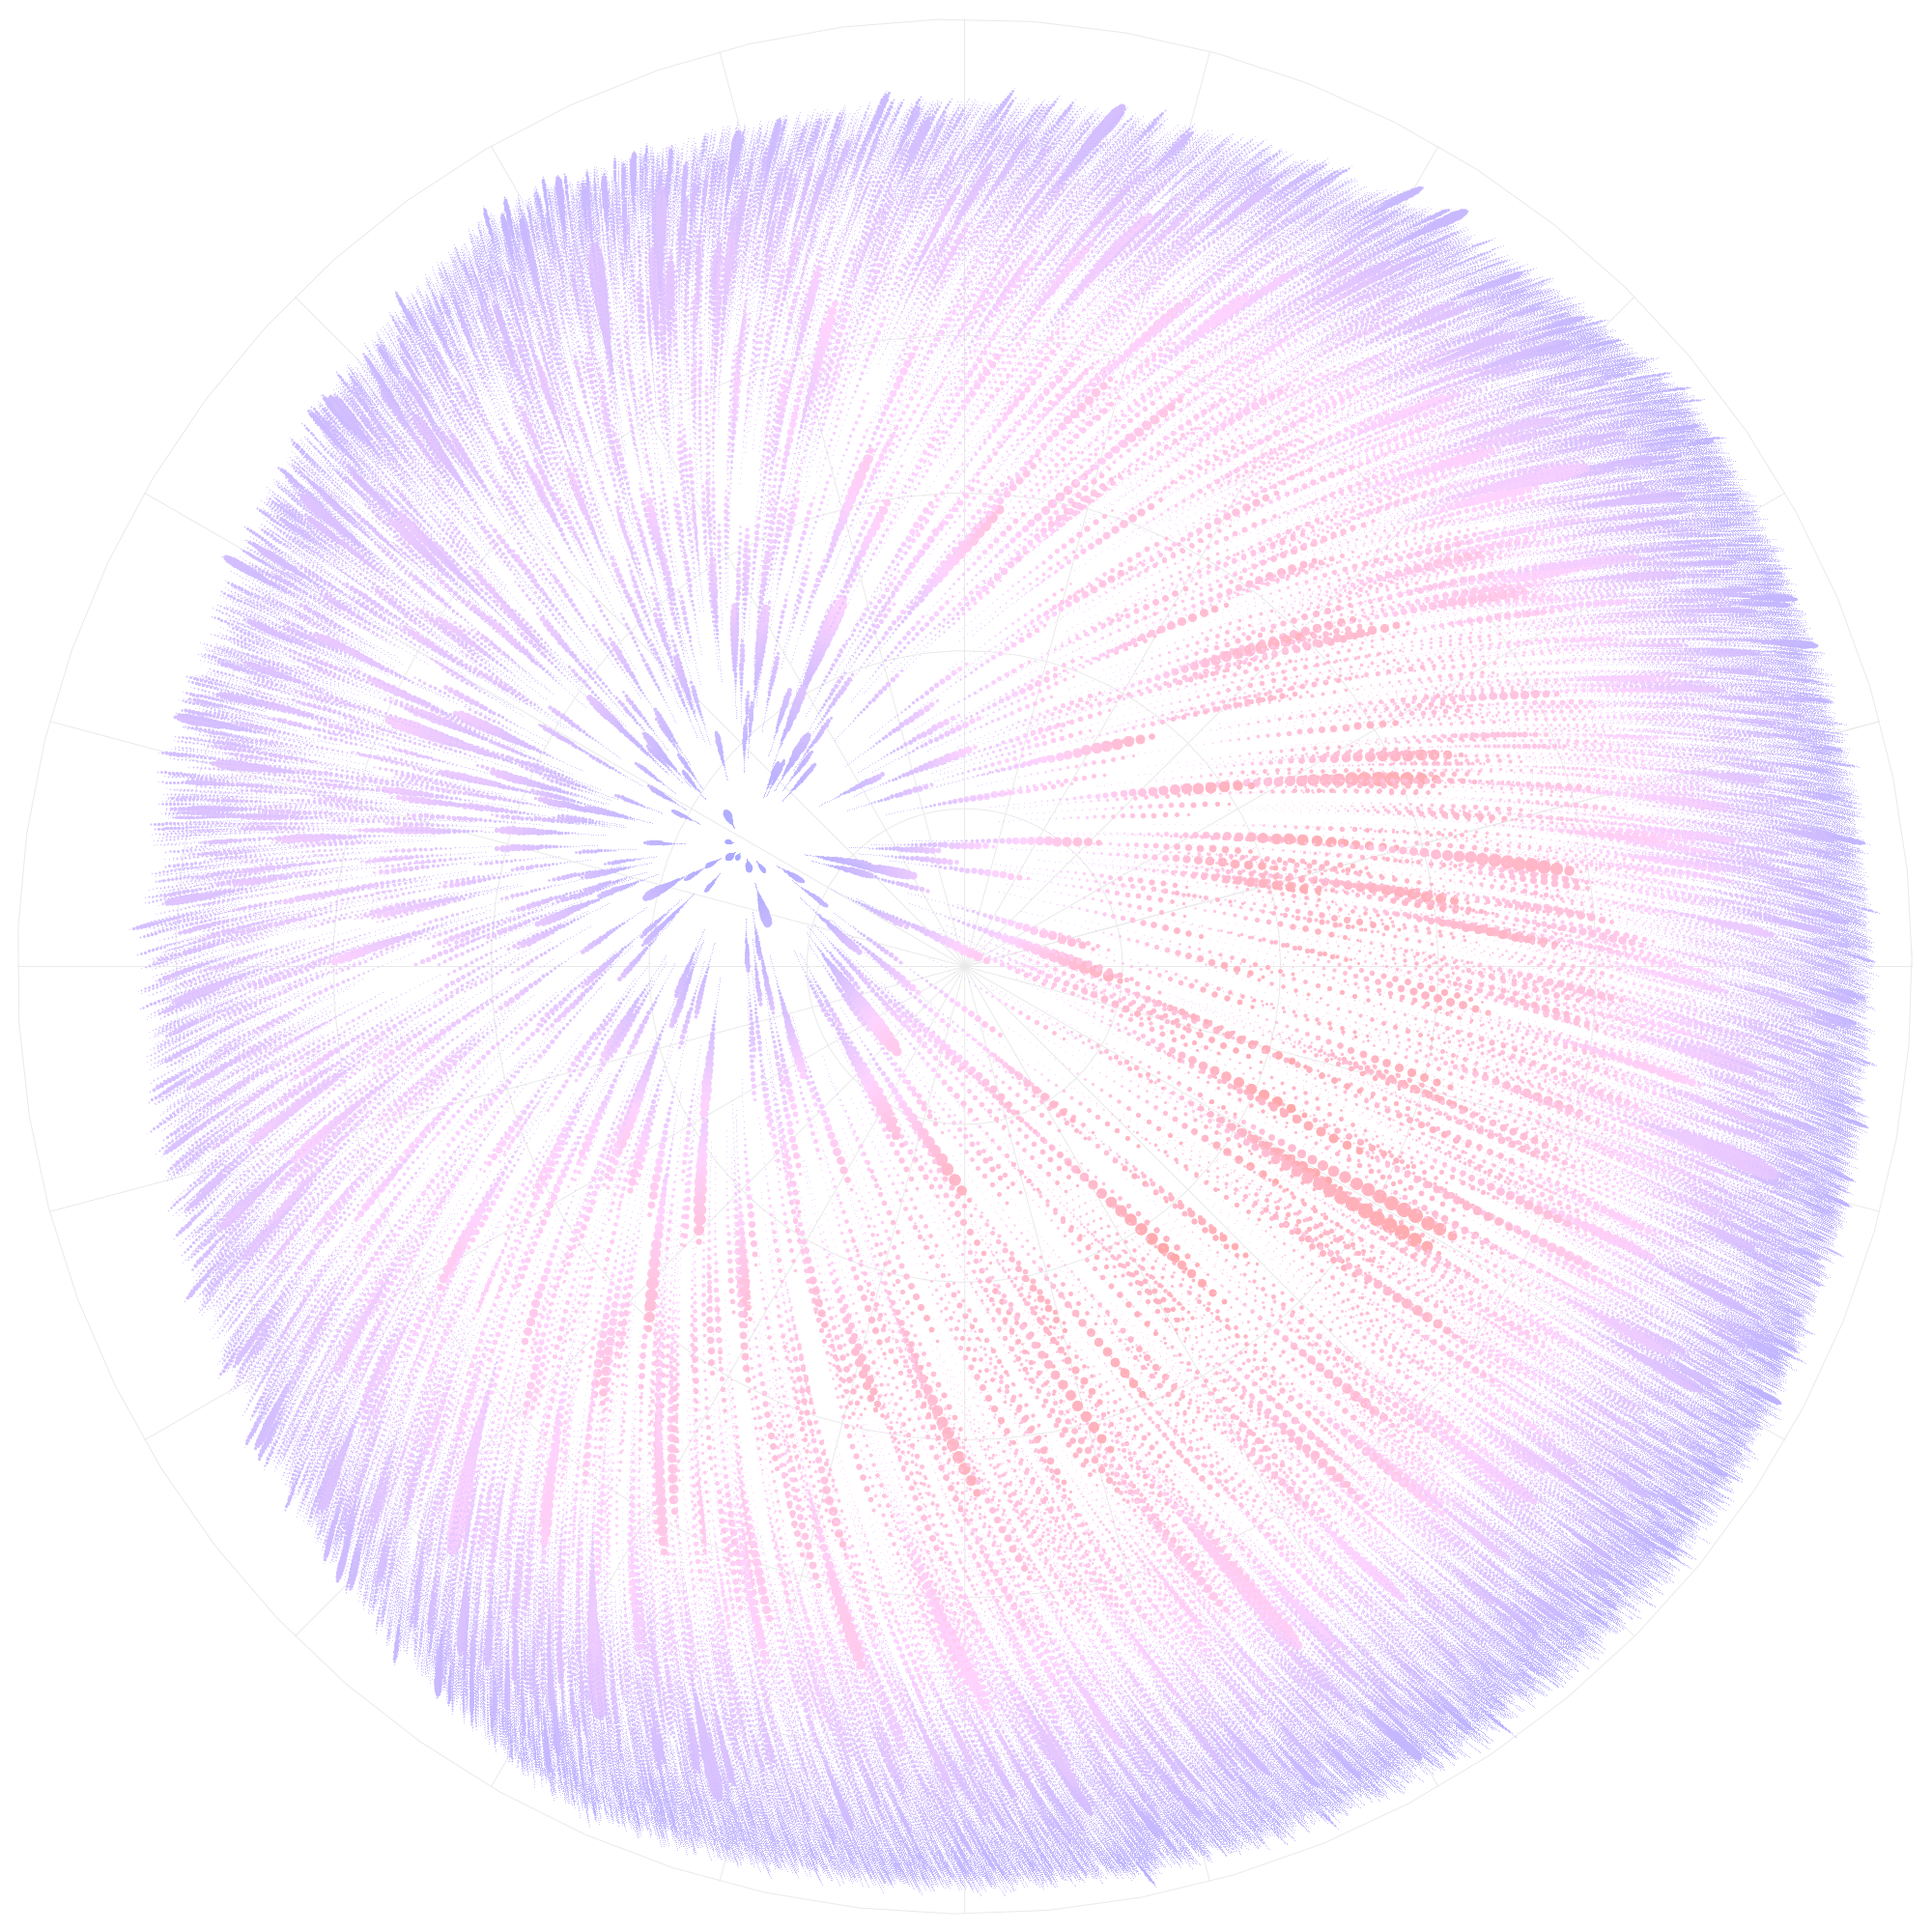
\includegraphics[width=\paperwidth]{fireworks-i.png}}
        \begin{frame}
            \titlepage
        \end{frame}
    }
                
    \section{Overview}
        \frejm{Motivation}{
            {\large All work and no play makes Jack a dull boy...}\\[10mm]
            \hfill \textit{English proverb}
        }

        \frejm{What do we have?}{
            \begin{itemize}
                \item a (more-or-less) universal meteor simulator
                \pause
                \item with it we can
                \begin{itemize}
                    \item estimate meteor flux
                    \item validate physical models
                    \item investigate $r$ and $s$ indices
                    \item ...
                \end{itemize}
            \end{itemize}
            \pause
            \begin{itemize}
                \item let's go beyond statistics
                \item look at variations in meteors' properties
            \end{itemize}
        }

        \frejm{Algorithm}{
            \begin{enumerate}
                \item generate the meteoroid population
                \begin{itemize}
                    \item how?
                \end{itemize}
                \pause
                \item simulate atmospheric entry
                \pause
                \item compute meteor sightings
                    \begin{itemize}
                        \item position in the sky
                        \item magnitude
                        \item entry angle
                        \item ...
                        \pause
                        \item \emph{anything}
                    \end{itemize}
                \pause
                \item look at the dataset
            \end{enumerate}
        }
						
    \setbeamersize{description width = 5mm}
    \section{Simulation}
         This time we are investigating the models
        \frejm{Model}{            
            \emph{Whipple} (1938), improved by \emph{Öpik} (1955) and \emph{Ceplecha} (2001)
            
            We assume
            \begin{itemize}
                \item spherical, continuously ablating particles
                \item continuous thermal ablation
                \item no ionization or trail emission
            \end{itemize}
            
            We need
            \begin{itemize}
                \item equations of motion
                \item equation of luminance
                \item atmospheric and instrumental effects
                \item to compute the statistic
            \end{itemize}            
        }
    
        \frejm{Equations of motion}{
            \begin{itemize}
                \item braking equation
                $$
                    \diff{v} = -\frac{\Gamma A}{m^{1/3} \rho^{2/3}} \rho_{\mathrm{air}} v^2 \diff{t}
                $$
                \item equation of ablation
                $$
                    \diff{m} = -\frac{\Lambda A}{2Q} \frac{m^{2/3}}{\rho^{2/3}} \rho_{\mathrm{air}} v^3 \diff{t}
                $$
                \item equation of luminance
                $$
                    L = \tau(v) \frac{\Lambda A}{4Q} \frac{m^{2/3}}{\rho^{2/3}} \rho_{\mathrm{air}} v^5
                $$
                \begin{itemize}
                    \item $\tau(v)$ determined by \emph{Jones \& Halliday (2001)}
                \end{itemize}
            \end{itemize}
        }
        
        \frejm{Simulation of flight}{
            Full \emph{3D simulation} on spherical Earth
            \begin{itemize}
                \item Runge--Kutta integrator
                \item \emph{snapshots} taken $N$ times per second
                \item until complete ablation (or...)
            \end{itemize}
        }
        
        \fspicture{loginitMass-elevation-appMag.png}[H]

    \section{Prerequisites}
        \frejm{Monte-Carlo generator}{
            \begin{itemize}
                \item approximate the real population
                \begin{itemize}
                    \item easy for \emph{showers}
                    \item \emph{very difficult} for sporadic background
                \end{itemize}
                \pause
                \item $\pm$ constant $\vec{v_{\infty}}$
                \item slowly varying activity
            \end{itemize}
        }

        \frejm{Grid generator}{
            Plain old scientific method:
            \pause
            \begin{itemize}
                \item fix all parameters of meteoroids...
                \pause
                \item ...except one...
                \pause
                \item ...vary it slowly
            \end{itemize}
            \vspace*{5mm}
            \pause
            \begin{itemize}
                \item simulate, observe, analyze...
                \item look for changes in the output
            \end{itemize}
            \vspace*{5mm}
            \pause
            We may look at the \emph{brightest frame} or \emph{entire trail}
        }
        
        \fspicture{real-sky.png}[H]
        \fspicture{grid-sky.png}[H]

        \frejm{Constraints}{
            We simplify things (unless stated otherwise)
            \pause
            \begin{itemize}                
                \item observer at North Pole
                \item constant atmospheric model
                \item start in zenith
            \end{itemize}
            \pause
            \begin{itemize}                
                \item scatter plot
                \item colour by varied property
                \item emphasize \emph{max-light frame}
            \end{itemize}
        }

        \frejm{What is it good for?}{
            \begin{itemize}
                \item improve ablation and flight models
                \item atmospheric tides
                \item try to find something interesting in the data
            \end{itemize}
        }

    \section{Entry angle}
        \frejm{Entry angle}{
            varying \emph{entry angle}
            \begin{itemize}
                \item Perseids
                \begin{itemize}
                    \item material, velocity, ...
                \end{itemize}
                \item mass \SI{1}{\gram}
                \item $\theta$ between \ang{10} and \ang{90}
            \end{itemize}
        }
        \fspicture{dec/thz.png}
        \fspicture{dec/tMz.png}
        \fspicture{dec/tmz.png}

    \section{Mass}
        \frejm{Parameters}{
            \begin{itemize}
                \item Perseids
                \begin{itemize}
                    \item material, velocity, ...
                \end{itemize}
                \pause
                \item entering atmosphere at \ang{45}
                \item $m_\infty$ from \SI{1}{\micro\gram} to \SI{1000}{\kilo\gram}
                \item log spacing
            \end{itemize}
        }
        \fspicture{mass/Mhu.png}

        \fspicture{mass/uQu.png}
        \frejm{Mass fraction at maxlight}{
            \begin{itemize}
                \item maximum brightness at $\approx$1/3 initial mass
                \item non-linear behaviour
            \end{itemize}
        }

        \fspicture{mass/tWu.png}
        \fspicture{mass/twu.png}
        \fspicture{mass/twu2.png}
        
    %\section{Ablation}
    %    \frejm{Heat of ablation}{
    %        varying \emph{enthalpy of vaporization} $Q$
    %        \begin{itemize}
    %            \item Perseids
    %            \item \SIrange[per-mode = symbol]{1e3}{1e8}{\joule\per\kilo\gram}
    %        \end{itemize}
    %    }
    %    \fspicture{ablationHeat/MhQ.png}

    %\section{Density}
    %    \frejm{Parameters}{
    %        \begin{itemize}
    %            \item vertical entry
    %            \item varying \emph{density} between \SIrange{200}{8000}{\kilo\gram\per\metre\cubed}
    %        \end{itemize}
    %    }
    %    %\fspicture{densities...}

    \section{Ultra-high entry velocity}
        \frejm{Ultra-high entry velocity}{
        Revise \emph{High geocentric velocity meteor ablation} (Hill et al., 2005)
            \begin{itemize}
                \item fluffy cometary material
                \item \emph{speed} between \SIrange{70}{500}{\kilo\metre\per\second}
                \item \emph{mass} between \SIrange{1e-12}{1e-6}{\kilo\gram}
            \end{itemize}
        }
        \fspicture{hv/grid.png}
        \fspicture{hv/Mhv.png}
        \fspicture{hv/thv.png}

        \frejm{Observations}{
            \begin{itemize}
                \item there are still no observations of such meteors
                \pause
                \item upper limit on flux
                \begin{itemize}
                    \item needs precise understanding of selection bias
                \end{itemize}
                \pause
                \item observation difficult
                \begin{itemize}
                    \item all-sky cameras
                    \item telescopes
                \end{itemize}
            \end{itemize}
        }

    \section{Conclusion}
        \frejm{Validation}{
            \begin{itemize}
                \item try to simulate real \emph{individual meteors}
                \item revise the physics in the model
                \begin{itemize}
                    \item does not take body heating into account
                    \item very simple light emission model
                    \item not sensitive to $\Gamma$
                \end{itemize}
            \end{itemize}
        }

        \frejm{Ultimate goal}{
            \begin{itemize}
                \item hopefully design a \emph{better model} of meteor flight
                \begin{itemize}
                    \item compare with real meteors                        
                    \item use in flux estimations
                \end{itemize}
            \end{itemize}
        }

        \frejm{Find motivation}{
            {\large ...all play and no work makes Jack a mere toy.}\\[10mm]
            \hfill \textit{Harry and Lucy Concluded} \\
            \hfill \textit{Maria Edgeworth (1825)}%
        }

        \frejm{Summary}{
            \begin{itemize}
                \item versatile, universal tool
                \item applicable to \emph{almost any} meteor observing system
            \end{itemize}
            \pause
            \begin{itemize}
                \item everything is \emph{open-source}
                \begin{itemize}
                    \item \url{https://github.com/sesquideus/asmodeus}
                \end{itemize}
                \item available for anyone (Python required)
                \pause
                \item suggestions or comments always welcome
            \end{itemize}
        }
        
        \frejm{References}{
            \begin{itemize}
                \item \textbf{Öpik, E. J.}:
                    Physics of meteor flight in the atmosphere. Interscience Publishers, 1958.  
                \item \textbf{Hill, K. A. -- Rogers, L. A. -- Hawkes, R. L.}:
                    High geocentric velocity meteor ablation. Astronomy \& Astrophysics 444, 615--624 (2005) 
                \item \textbf{Jones, W. -- Halliday, I.}:
                    Effects of Excitation and Ionization in Meteor Trains. MNRAS vol. 321, 2001, pp417--423.
            \end{itemize}
        }
            
\end{document}
